\chapter{A golyók pozíciójának felismerése}
\section{A probléma ismertetése}
Ebben a fejezetben a címből is láthatóan az asztal és azon elhelyezkedő \textbf{golyók pozíciójának felismeréséről} lesz szó. A program ezen része bemenetként fog fogadni egy képet. Ez a kép származhat \textbf{videófelvételből} (videófelvétel egy képkockája), \textbf{valós idejű felvételből} (szintén egy képkocka), vagy szimplán egy \textbf{képfájlból}. A program készítése közben egy valósághű internetes snooker játékról\cite{flyordie} készített felvételeket fogok használni a felismeréshez. A videójátékból származó felvétel azonban bizonyos szempontokból eltér a valóságtól, ezekről később lesz szó, de lényegében jól használható a felismerés elkészítéséhez, továbbá megkönnyíti a tesztelést és a felvételek beszerzését. A bemenő adatot ezután képfelismerési folyamatok után a \ref{tab:felismert_koordinatak} táblázatban látható koordinátákra alakítjuk.

\begin{figure}[!ht]
    \centering
    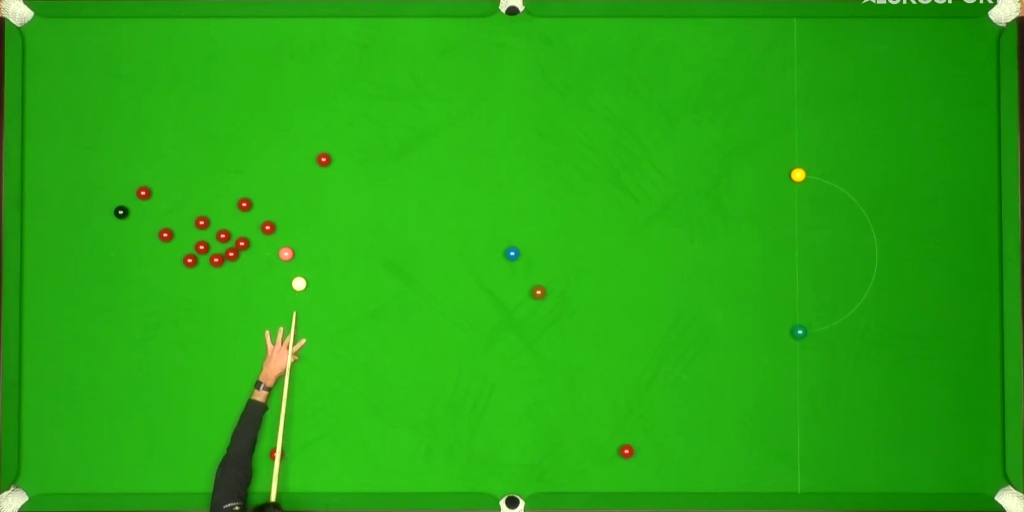
\includegraphics[width=100mm, keepaspectratio]{figures/input_table.png}
    \caption{Egy bemeneti kép az asztal felismerő lépés után.}
    \label{fig:bemeneti_asztal}
\end{figure}

\begin{table}[!ht]
    \caption{A golyó felismerés kimeneti adatai a \ref{fig:bemeneti_asztal} kép alapján.}
    \label{tab:felismert_koordinatak}
	\footnotesize
	\centering
	\begin{tabular}{ l l l }
		\toprule
		golyó színe & x pozíció (0 - 1024) & y pozíció (0 - 512) \\
		\midrule
		yellow & 156 & 176\\
        brown  & 224 & 254\\
        green  & 226 & 178\\
        red    & 460 & 480\\
        pink   & 464 & 344\\
        blue   & 514 & 256\\
        white  & 622 & 472\\
        red    & 698 & 324\\
        red    & 724 & 394\\
        red    & 896 & 250\\
        black  & 918 & 256\\
		\bottomrule
	\end{tabular}
\end{table}

\par A \ref{fig:bemeneti_asztal} képen már az asztal felismerés után való képet mutatom, a láthatóság megkönnyítése érdekében. A fejezet következő részeiben a bemeneti nyers képről koordinátákra való átalakítás lehetséges módszereit ismertetem lépésekre bontva.

\section{Az asztal felismerése}
Ez a lépés kicsit elkülönül a többi lépéstől, hiszen a további lépések különféle módszerektől függetlenül, megegyezően ezen a lépésen alapszanak. Ahhoz hogy a további lépések pontosak legyenek és megfeleő teljesítménnyel működjenek, az asztalt mindig azonos méretben, elforgatásban és torzításban kell megkapniuk.
\par Ebben a módszerben az elforgatáson kívül a detektálás, átméretezés és a torzítás lesz középpontban. Az elforgatást nem veszem figyelembe, hiszen a bemenetről elvárt, hogy bizonyos orientációban kapjuk meg. Tehát amit valójában kapunk függetlenül a bemenet megszerzésének módszerétől, a \ref{fig:bemeneti_kep} képen látható.

\begin{figure}[!ht]
    \centering
    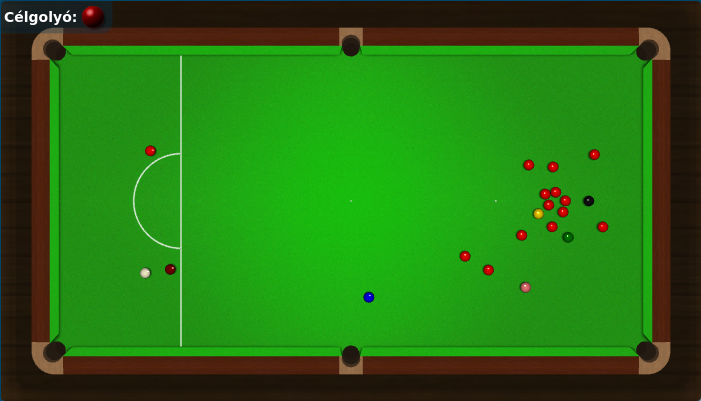
\includegraphics[width=150mm, keepaspectratio]{figures/input_screen.png}
    \caption{Egy nyers bemeneti kép a játék ablakáról.}
    \label{fig:bemeneti_kep}
\end{figure}

\par Ezen a képen kell megtalálnunk a játékterület zöld részét. Ezt megtehetjük, ha először is a képünket ún. HSV (Hue Saturation Value) formátumra alakítjuk. Ennek a konverziónak a kimenete a \ref{fig:bemeneti_kep_hsv} képen látható.

\begin{figure}[!ht]
    \centering
    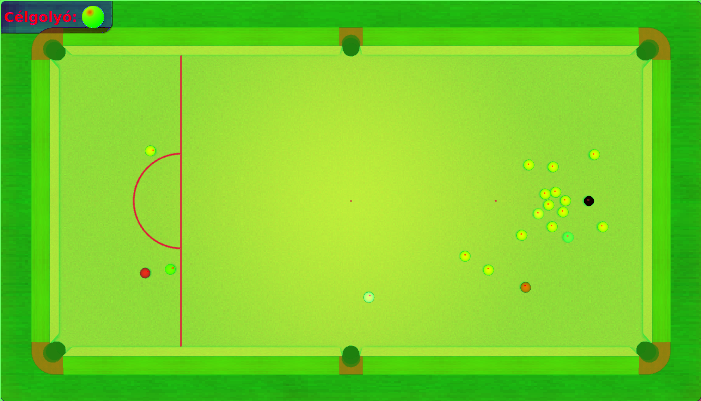
\includegraphics[width=150mm, keepaspectratio]{figures/input_screen_hsv.png}
    \caption{A \ref{fig:bemeneti_kep} kép HSV re alakított verziója RGB reprezentációban.}
    \label{fig:bemeneti_kep_hsv}
\end{figure}

\par Ez az átalakítás azért fontos, mert HSV formátumban könnyebben intervallumok közé lehet szorítani a játékterület zöld színét.
\newline Ezek az intervallumok:
\begin{itemize}
    \setlength\itemsep{-2pt}
    \item Árnyalat (Hue)
    \item Telítettség (Saturation)
    \item Érték (Value)
\end{itemize}
\par Az adott intervallum értékeken kívül helyezkedő értékeket maszkoljuk, és eredményül a kívánt zöld területeket kapjuk. Ezt a képet a maszkolás után visszaalakítjuk RGB formátumra. A folyamat után kapott kép a \ref{fig:bemeneti_kep_mask} képen látható.

\begin{figure}[!ht]
    \centering
    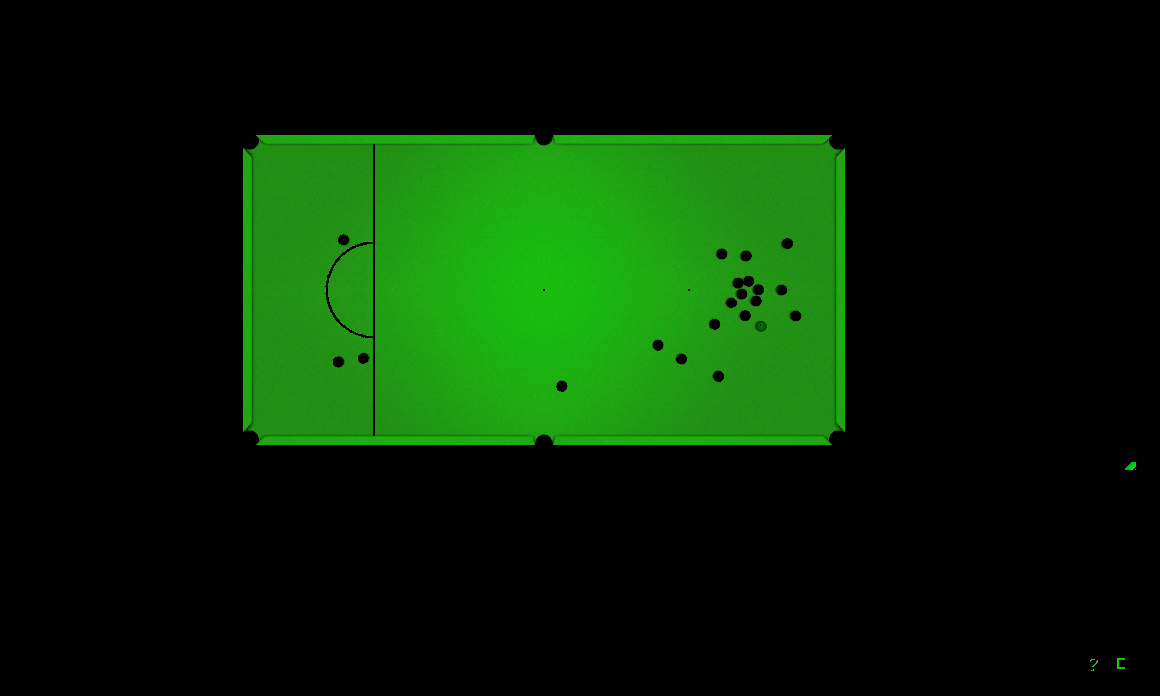
\includegraphics[width=150mm, keepaspectratio]{figures/input_screen_mask.png}
    \caption{A \ref{fig:bemeneti_kep} kép a maszkolás után.}
    \label{fig:bemeneti_kep_mask}
\end{figure}

\par Az előző folyamat után már jól látható a játékterület, azonban vannak apró foltok amik nem kerületk maszkolásra. Ezek a foltok hasonló HSV értékekkel rendelkeznek, mint a játékterület, kiszűrésük megoldható a kontúrok megkeresésével, majd feltételezve, hogy a legnagyobb folt a maszkolt képen a játékterület, annak kiválasztásával. Ezzel az eljárással már megadható a játékterület kontúrja. Feltételezve, hogy ez a négy sarokpontból áll, és egy téglalap pontosan határolja, a játékterület képe \ref{fig:bemeneti_asztal2} megkapható a kontúr eredeti képből való kivágásával és átméretezésével.

\begin{figure}[!ht]
    \centering
    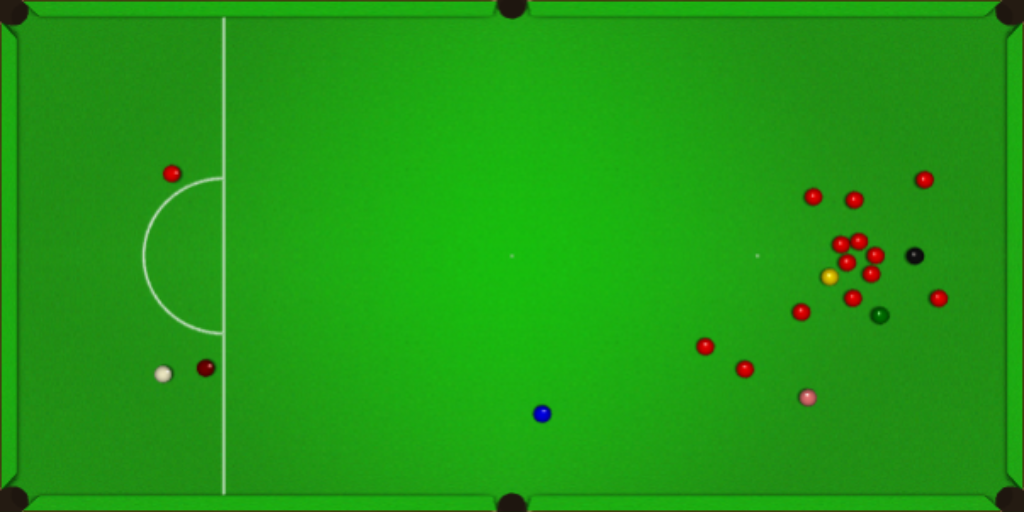
\includegraphics[width=100mm, keepaspectratio]{figures/input_table2.png}
    \caption{Az eredeti képből kinyert játékterület.}
    \label{fig:bemeneti_asztal2}
\end{figure}

\par Fent említettem, hogy feltételezhetjük, hogy a játékterület kontúrja a kontúrkeresés után téglalap alakú, és a kontúrt alkotó pontok száma 4. Viszont valóságban ez nehezen fordul elő, ezért szükséges a pontok számának leszűkítése és a négy pontot határoló alakzatban lévő kép torzítása 2:1 oldalarányú téglalapra. Az oldalarány a szabvány snookerasztal 12 x 6 láb (365,8 cm x 182,9 cm)\cite{snooker_rules} méretéből következik. A pontok szűkítéséről és a torzításról a megvalósítás fejezetben lesz részletesetbben szó.

\section{A golyók azonosítása}
A golyók azonosítását különféle mószerekkel végezhetjük el, ezek eltérnek sebességben és pontosságban. A folyamatok bemenete az előzőekben megismert asztal felismerés kimenete lesz, kimenetük pedig a \ref{tab:felismert_koordinatak} táblázatban látható x és y pozíciók, adott golyók színe szerint. A folyamat belső működése módszerenként eltér egymástól, ezeket a módszereket az implementáció egyes iterációjának részeként használtam, majd változtattam meg az elért teljesítmény növeléséhez.

\subsection{Azonosítás mintaillesztéssel}
Ennek a módszernek az alapja tisztán mintaillesztéssel működik. A mintaillesztés egy arányos méretű képet illeszt rá a játékterület képére, majd amennyiben az illeszkedés mértéke meghalad egy bizonyos küszöbértéket, a mintaillesztés iterációjának a pozíciója mentésre kerül. Ebből a pozícióból meghatározható a golyó helyzete. A mintaillesztéshez használt minta a \ref{fig:minta_kep} ábrán látható.

\begin{figure}[!ht]
    \centering
    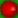
\includegraphics[width=30mm, keepaspectratio]{figures/template_red.png}
    \caption{A mintaillesztéshez használt minta.}
    \label{fig:minta_kep}
\end{figure}

\par A \ref{fig:minta_kep} minta felbontása láthatóan alacsony, azonban túl nagy felbontás esetén a folyamat meglehetősen lassabban megy végbe, továbbá a minta méretét még a felismert játékterület mérete is meghatározza.
\par A mintaillesztés ún. Kereszt Korrelációval (Normed Cross Correlation) megy végbe, ezt a \ref{for:cross_correlation} képletben láthatjuk\cite{template_match}.

\begin{equation}
    R(x, y) = \frac{\sum_{x',y'}(T(x',y') \cdot I(x + x', y + y'))}{\sqrt{\sum_{x',y'}T(x',y')^2 \cdot \sum_{x',y'}I(x + x',y + y')^2}}
    \label{for:cross_correlation}
\end{equation}

\par A képletben az $x$ és $y$ az eredeti képen vizsgált terület bal felső sarkát, $x'$ és $y'$ a minta képnek az adott képpontját, $T$ a minta képet és $I$ az eredeti képet jelöli.
\par A mintaillesztés problémái közé tartozik, hogy a zöld golyó mintaillesztésénél a küszöbérték et beállítani nehéz, és az eredmény pontatlan, lásd \ref{fig:rossz_zold}.

\begin{figure}[!ht]
    \centering
    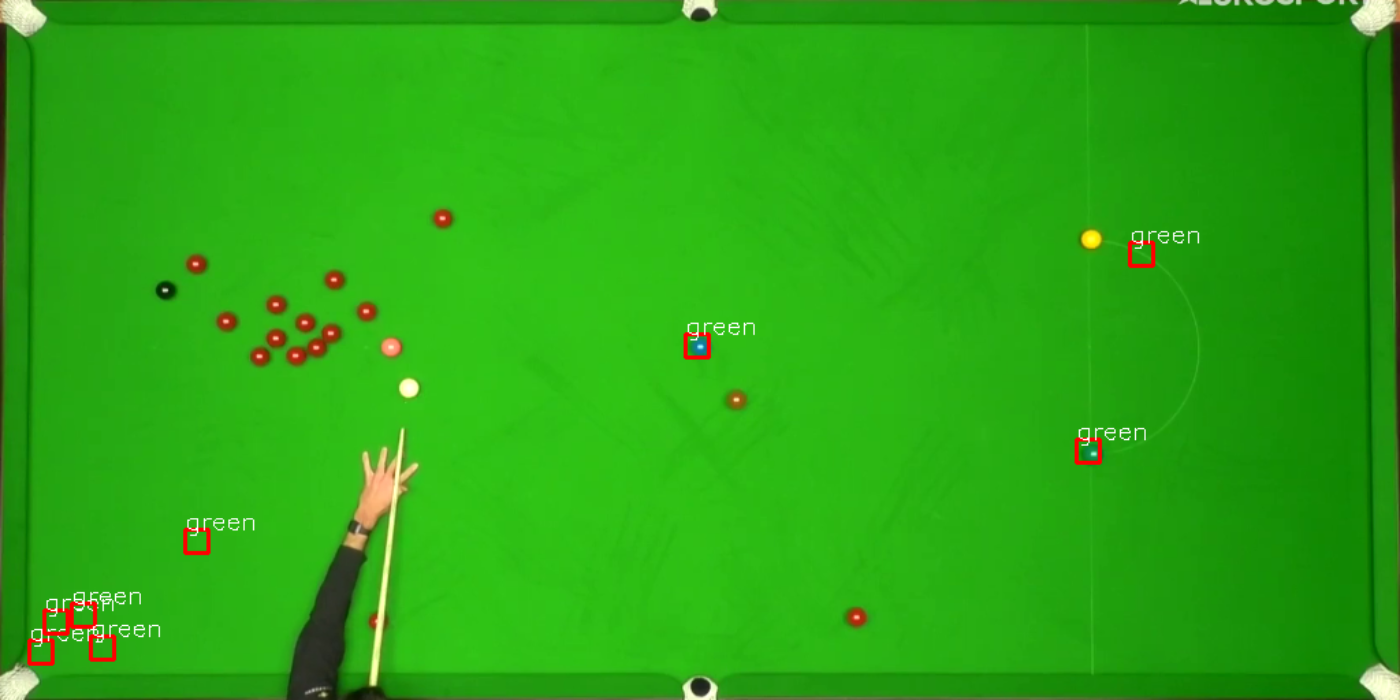
\includegraphics[width=73mm, keepaspectratio]{figures/wrong_green.png}\hspace{2mm}
	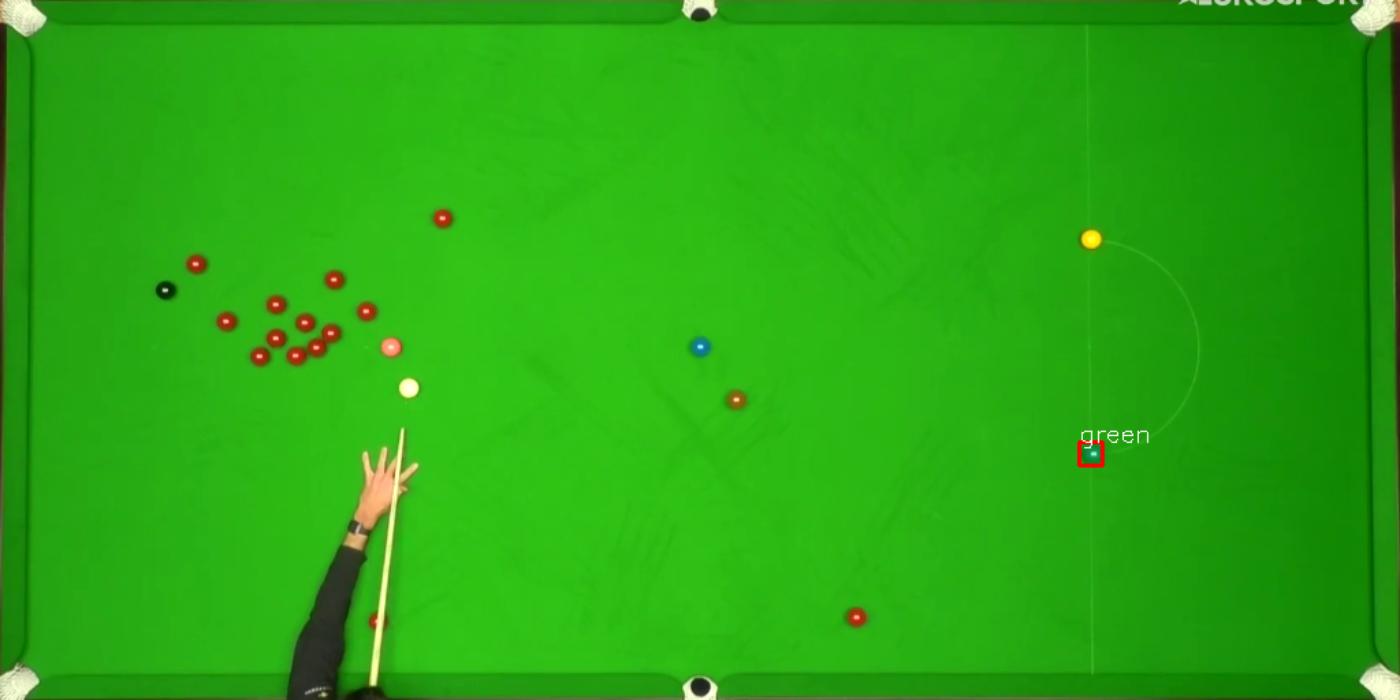
\includegraphics[width=73mm, keepaspectratio]{figures/green_ok.png}\\\vspace{5mm}
    \caption{A zöld golyó mintaillesztésének hibája (bal) és annak orvoslása HSV konverzióval (jobb).}
    \label{fig:rossz_zold}
\end{figure}

\par A \ref{fig:rossz_zold} ábrán látható hiba valamelyes orvosolható a kép és minta HSV -re való konvertálásával. Ez a konverzió jó eredményeket ad, azonban nagyon minimálisan csökkenti a teljesítményt. A mintaillesztés sajnos prolémákba ütközik a piros és barna golyók megkülönböztetésekor is. Ez a \ref{fig:rossz_barna} képen látható.

\begin{figure}[!ht]
    \centering
    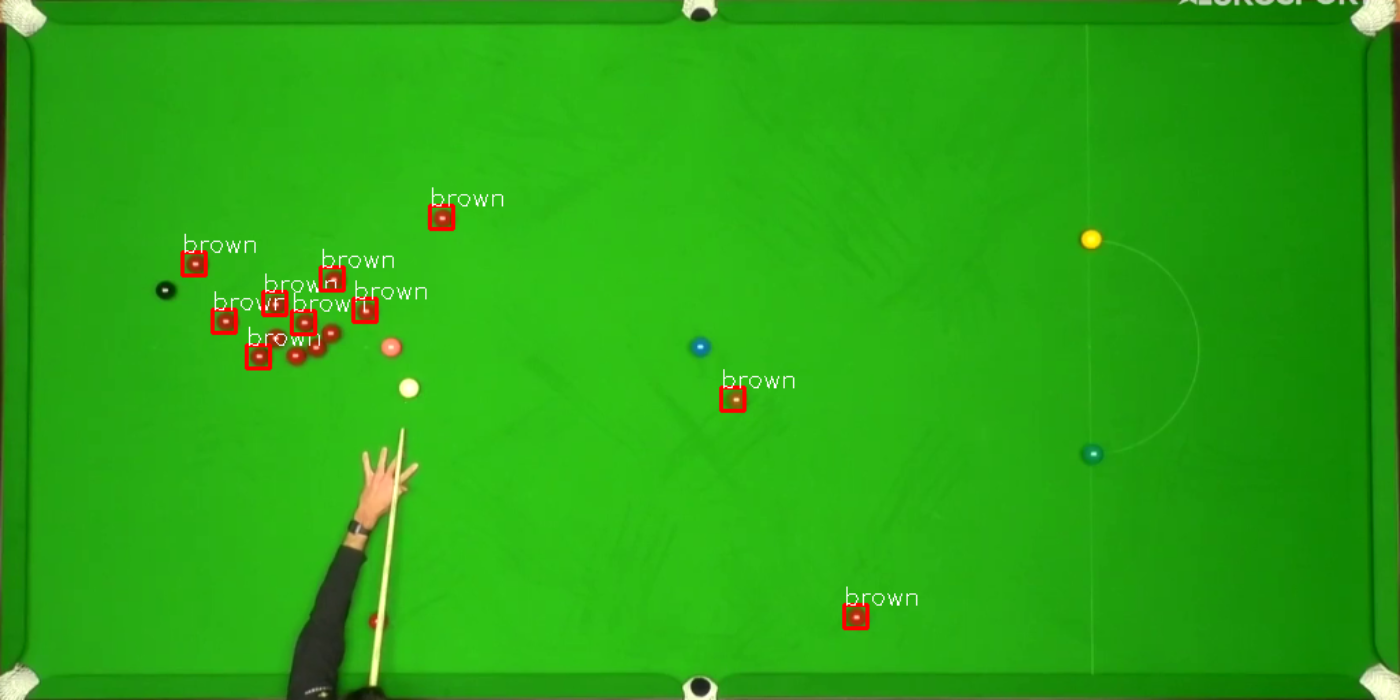
\includegraphics[width=73mm, keepaspectratio]{figures/wrong_brown.png}\hspace{2mm}
	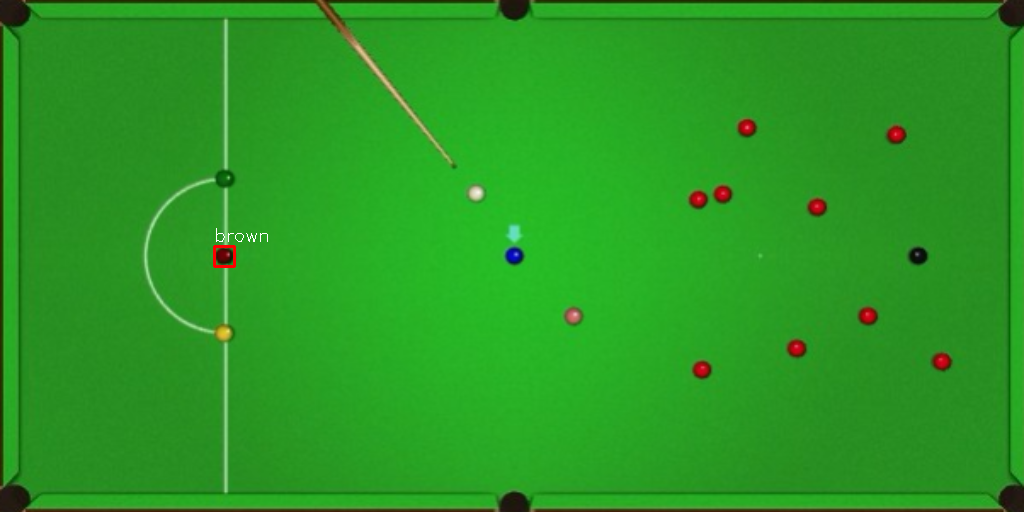
\includegraphics[width=73mm, keepaspectratio]{figures/brown_ok.png}\\\vspace{5mm}
    \caption{A barna golyó mintaillesztésének hibája (bal) és annak orvoslása a piros golyók levonásával (jobb).}
    \label{fig:rossz_barna}
\end{figure}

\par Itt a színek közelsége miatt nehéz megkülönböztetni a golyókat, ezért a piros és barna golyók nagyon minimálisan térnek el a \ref{for:cross_correlation} függvény miatt. Ez a probléma HSV konvertálás után is fennáll. Erre a megoldás, hogy az érzékelt piros golyók kivonásra kerülnek a barna golyók listájából. Ahhoz, hogy pontos legyen az eredmény, viszont szükséges, hogy a piros golyók megfelelően legyenek érzékelve, amely nem minden esetben biztosítható, ezért ez a módszer nem túl pontos bizonyos bemenetekre. Hasonló problémák merülhetnek fel a piros és rózsaszín, továbbá a fehér és rózsaszín golyók felismerésekor is.
\par Annak ellenére, hogy a módszer nem túl optimális, jól használható adatkészeletek készítésére, hiszen a felsmerést nagyrészt helyesen megoldja és a problémák ismeretében a kézzel válogatást nagymértékben megkönnyíti.

\subsection{Azonosítás körkeresés és mintaillesztéssel}
Az előző módszerhez hasonlóan a golyó színek szerinti osztályozása itt is mintaillesztéssel történik, azonban a sebesség növelése érdekében itt először a golyókat kördetektálással azonosítjuk, majd ennek eredményét adjuk át a mintaillesztő algoritmusnak. Ez az egész képen való pásztázás és mintaillesztéshez képest a teljesítményt a minták leszűkített mennyiségével nagymértékben növeli.

\par A körök detektálásához az ún. Hough transzformációt (Hough Transformation) fogom használni, ez a H.K. Yuen, J. Princen, J. Illingworth és J. Kittler et. al. 1990 \cite{YUEN199071} szerint abban az esetben, ha egy kör a kövekező \ref{for:hough_transform} függvénnyel írható le,

\begin{equation}
    (x - a)^2 + (y - b)^2 = r^2
    \label{for:hough_transform}
\end{equation}

\par ahol $a$ és $b$ a kör középpontjának koordinátái és $r$ a sugár, akkor a körvonal élének egy tetszőleges $x_i$, $y_i$ pontja átalakításra kerül egy $a$, $b$, $r$ paraméterek által meghatározott térben elhelyezkedő egyenes kör alapú kúppá.\cite{hough_transform,YUEN199071} Amennyiben az adott pontok egy körvonalon helyezkednek el, a kúpok metszeni fogják egymást a kör $a$, $b$, $r$ pontjainak megfelelően.\cite{YUEN199071}
\par A körök megtalálásához az algoritmusnak meg kell adni néhány paramétert, ezek közé tartozhat:
\begin{itemize}
    \setlength\itemsep{-2pt}
    \item A keresett körök minimális és maximális sugara
    \item A keresett körök közti minimális távolság, duplikációk szűréséhez
    \item Az ellenőrzött alakzatok körrel való hasonlóságának küszöbértéke
\end{itemize}
\par Az algoritmus lefutása után megkapjuk a bemeneti játékterületen talált kör alakú kontúrokat. Ezt a \ref{fig:talalt_korok} ábra szemlélteti.

\begin{figure}[!ht]
    \centering
    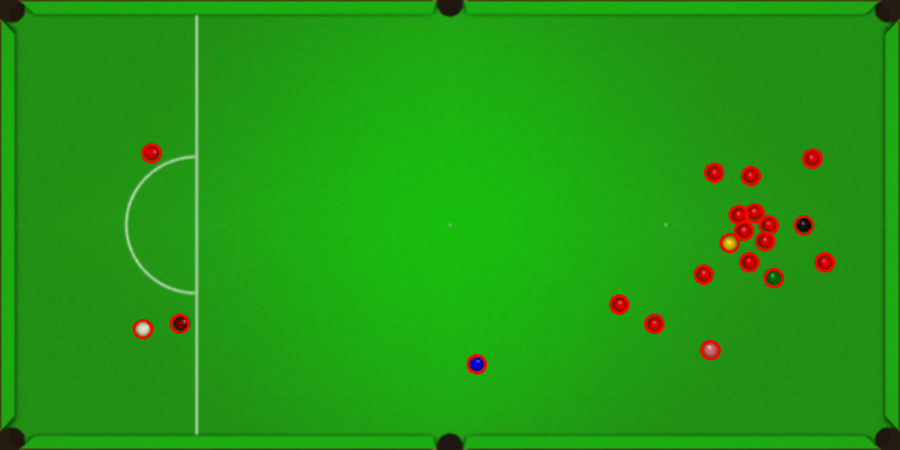
\includegraphics[width=100mm, keepaspectratio]{figures/detected_circles.png}
    \caption{A Hough transzformáció lefutása után kapott körök.}
    \label{fig:talalt_korok}
\end{figure}

\par Ez a módszer körök megtalálására jól használható, a mintaillesztéshez szükséges képek könnyedén kivághatók az eredeti képből a körök paraméterei alapján. A probléma szintén a mintaillesztéssel van, hiszen a kivágott körök az előzőleg megismert mintaillesztéssel kerülnek beazonosításra. Ez sajnos az eddig megismert hibákat vonja maga után, annak ellenére, hogy a sebesség javul. Viszont akárcsak a szimpla mintaillesztéses módszer ez a módszer is alkalmas adatkészletek elkészítésére, és a kapott adatok kézzel ellenőrzését nagymértékben megkönnyíti.

\subsection{Azonosítás körkeresés és gépi tanulás segítségével}
Ahhoz, hogy kiküszöböljük a mintaillesztés hibáit, az osztályozást elvégezhetjük neurális hálózat segítségével. Ezt megtehetjük ugyancsak, ha egy kerettel végigpásztázunk a játékterület képén, de a körkereséses módszernél megismert Hough transzformációval jobb eredményt is elérhetünk. A következőkben a körkeresés eredményeképp kapott, a bemeneti játékterület képéből kivágott golyók osztályozásáról lesz szó neurális hálózat segítségével. A kivágott képek fogják a bemenetet képezni, majd a neurális hálózat azt osztályozza egy 0 tól 7 ig terjedő egész számként. Ezek a számok a golyók színeit reprezentálják, lásd \ref{tab:golyo_azonositok} táblázat.

\begin{table}[!ht]
    \caption{A golyók szín szerint, és azok azonosítói.}
    \label{tab:golyo_azonositok}
	\footnotesize
	\centering
	\begin{tabular}{ l c }
		\toprule
		Golyó színe & Azonosító \\
		\midrule
		fekete      & 0\\
        kék         & 1\\
        barna       & 2\\
        zöld        & 3\\
        rózsaszín   & 4\\
        piros       & 5\\
        fehér       & 6\\
        sárga       & 7\\
		\bottomrule
	\end{tabular}
\end{table}

\par A neurális hálózat betanításához szükség van betanítási adatkészletre, viszont az előzőekben megsimert módszereknél szóba került, hogy viszonylag kevés kézi szortírozással könnyedén lehet velül előállítani adatkészletet, amely tökéletes a neurális hálózat betanításához és teszteléséhez. Az adatkészlet néhány eleme látható a \ref{fig:adatkeszlet} ábrán.

\begin{figure}[!ht]
    \centering
    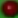
\includegraphics[width=30mm, keepaspectratio]{figures/dataset_1.png}\hspace{5mm}
    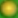
\includegraphics[width=30mm, keepaspectratio]{figures/dataset_2.png}\hspace{5mm}
	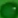
\includegraphics[width=30mm, keepaspectratio]{figures/dataset_3.png}\\\vspace{5mm}
    
\includegraphics[width=30mm, keepaspectratio]{figures/dataset_4.png}\hspace{5mm}
    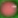
\includegraphics[width=30mm, keepaspectratio]{figures/dataset_5.png}\hspace{5mm}
	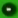
\includegraphics[width=30mm, keepaspectratio]{figures/dataset_6.png}\\\vspace{5mm}
    \caption{Az adatkészlet elemei.}
    \label{fig:adatkeszlet}
\end{figure}

\par A betöltött adatokat megfelelően azonosítva címkéjük szerint, átadjuk a neurális hálózatnak. Ahhoz, hogy a tanítás jó eredményeket hozzon, gondoskodni kell arról, hogy a betanítási adatok közt egyenlő arányban szerepelnek az egyes golyók színek szerint, továbbá, hogy az adatkészlet elemei megfelelően össze vannak keverve. Az előkészített adatkészlet egy kis részét (10\% - 30\%) elkülönítjük, majd ezt használjuk a neurális hálózat pontosságának tesztelésére.
\par A betanítási folyamatok után elmentjük a neurális hálózatot, majd amikor használni szeretnénk, csak be kell tölteni. A tanítás és felhasználás külön programfájlokban könnyedén elvégezhető.
\par A körfelismerés módszerrel ötvözve, a neurális hálózattal való osztályozás gyors és pontos eredményeket biztosít. A felismerés egy kimenetele a \ref{fig:felismert_asztal} képen látható.

\begin{figure}[!ht]
    \centering
    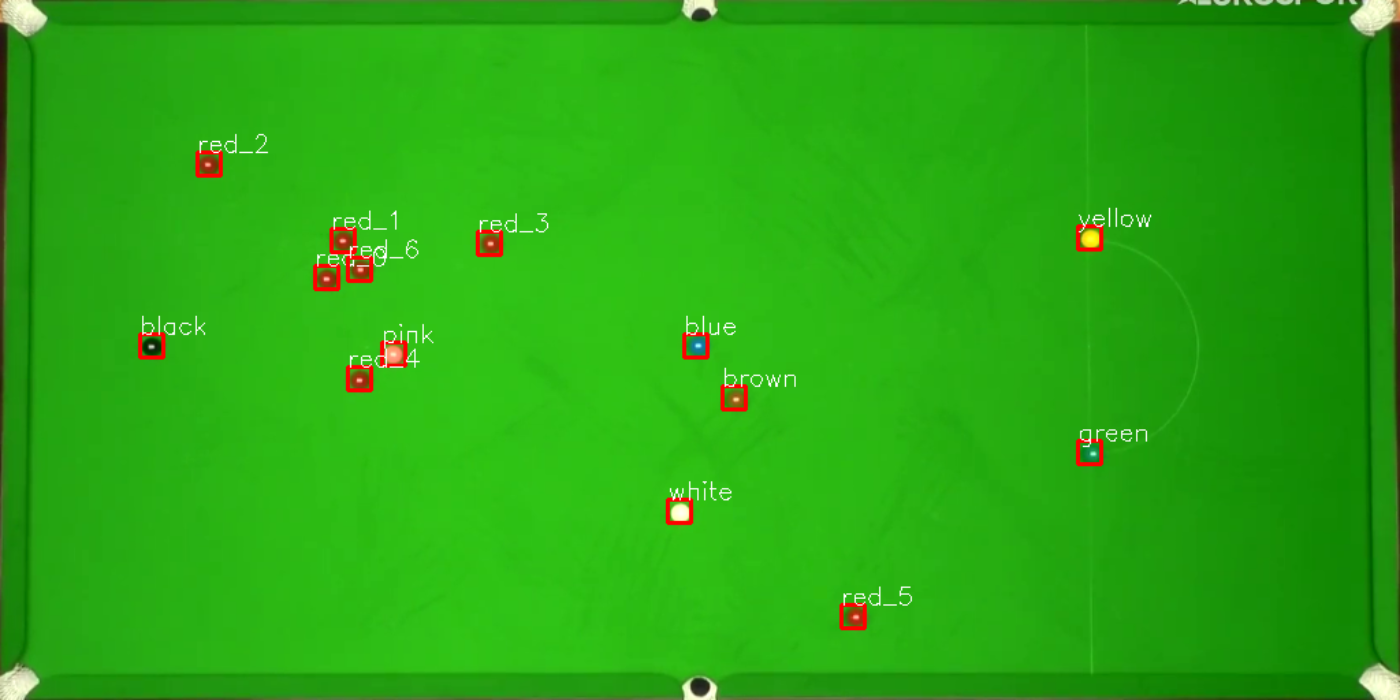
\includegraphics[width=100mm, keepaspectratio]{figures/recognised_table.png}
    \caption{A neurális hálózattal való golyófelismerés kimenete.}
    \label{fig:felismert_asztal}
\end{figure}

\par A módszer eredményességének köszönhetően későbbiekben részletesebben ismertetem a megvalósítás fejezetben.